\documentclass{beamer}

\usepackage{graphicx,multicol}
\usepackage{beamerouterthememiniframes, beamercolorthemeann,srcltx,hyperref}
\usepackage{listings}

\setbeamercolor{normal text}{fg=black!70}
\setbeamertemplate{navigation symbols}{}%geen navigatie
\setbeamertemplate{blocks}[rounded][shadow=true]
\setbeamertemplate{footline}{%
\hspace*{-0.5cm} \raisebox{5pt}{\makebox[\paperwidth]{\hfill\makebox[10pt]{\scriptsize\insertframenumber}}}}
 
\setbeamertemplate{caption}{\raggedright\insertcaption\par}

\title{Meta-tracing JIT compilation}
\author{Maarten Vandercammen}
\date{}

\lstset{
  language=Scheme
}

\begin{document}

\begin{frame}[plain]

\includegraphics[width=0.4\paperwidth]{VUB_logo.jpg}
\vspace{2cm}
\titlepage
\end{frame}

\begin{frame}[fragile]{Merging}
\hspace{2.2cm}
\only<1>{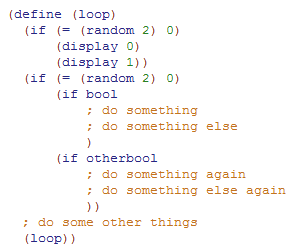
\includegraphics[scale=1]{merging_ex_1.png}}
\only<2>{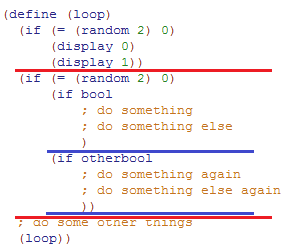
\includegraphics[scale=1]{merging_ex_2.png}}
\end{frame}

\begin{frame}[fragile]{Merging annotations}
\begin{lstlisting}[basicstyle = \small\ttfamily, escapechar = £]
(splits-control-flow)

(merges-control-flow)
\end{lstlisting}
\end{frame}

\begin{frame}[fragile]{Merging annotations}
\begin{lstlisting}[basicstyle = \scriptsize\ttfamily, escapechar = £]
(define (evaluate-if predicate consequent . alternate)
 (let* ((cond (evaluate predicate)))
   (splits-control-flow)
   (if cond
       (return-from-control-flow-split (thunkify consequent))
       (if (null? alternate)
           (return-from-control-flow-split £'£())
           (return-from-control-flow-split (thunkify (car alternate)))))))

(define (return-from-control-flow-split value)
   (merges-control-flow)
   value)
\end{lstlisting}
\end{frame}

\begin{frame}[fragile]{Handling annotations}
\begin{lstlisting}[basicstyle = \scriptsize\ttfamily, escapechar = £]
(define (step* state)
  (match state
    ((ko (haltk) _)
     v)
    ; evaluate annotations in step* instead of step
    ; annotations might not lead to recursive call to step*
    ((ev `(splits-control-flow) (cons £\scriptsize$\phi$£ £\scriptsize$\kappa$£))
     (handle-splits-cf-annotation (ko £\scriptsize$\phi$£ £\scriptsize$\kappa$£)))
    ((ev `(merges-control-flow) (cons £\scriptsize$\phi$£ £\scriptsize$\kappa$£))
     (handle-merges-cf-annotation (ko £\scriptsize$\phi$£ £\scriptsize$\kappa$£)))
    ((ko (can-close-loopk) (cons £\scriptsize$\phi$£ £\scriptsize$\kappa$£))
     (handle-can-close-loop-annotation v (ko £\scriptsize$\phi$£ £\scriptsize$\kappa$£)))
    ((ko (can-start-loopk £'£() debug-info) (cons £\scriptsize$\phi$£ £\scriptsize$\kappa$£))
     (handle-can-start-loop-annotation v debug-info (ko £\scriptsize$\phi$£ £\scriptsize$\kappa$£)))
    (_
     (let ((new-state (step state)))
       (step* new-state)))))
\end{lstlisting}
\end{frame}

\begin{frame}[fragile]{splits-cf-id stack}
\begin{lstlisting}[basicstyle = \scriptsize\ttfamily, escapechar = £]
(struct tracer-context (...
                        splits-cf-id-stack
                        ...))
                        
(define (handle-splits-cf-annotation state)
  (execute/trace `(pop-continuation)
                 `(push-splits-cf-id! ,(inc-splits-cf-id!)))
  (step* state))
  
(define (handle-merges-cf-annotation continuation)
  (let ((mp-id (pop-splits-cf-id!)))
    ...))
\end{lstlisting}
\end{frame}

\begin{frame}[fragile]{Use common trace for merging}
\hspace{2.2cm}
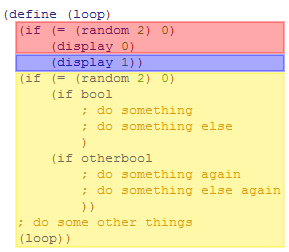
\includegraphics[scale=1]{merging_ex_3.png} 
\end{frame}

\begin{frame}[fragile]{Jumping to MP-tail-traces}
\begin{lstlisting}[basicstyle = \small\ttfamily, escapechar = £]
(letrec ((non-loop (lambda ()
           ; trace instructions
           (execute-mp-tail-trace id)))
   (non-loop))
   
(struct tracer-context (...
                        mp-tails-dictionary
                        ...)
\end{lstlisting}
\end{frame}

\begin{frame}[fragile]{Starting tracing}
\begin{lstlisting}[basicstyle = \tiny\ttfamily, escapechar = £]
(define (handle-merges-cf-annotation continuation)
  (let ((mp-id (top-splits-cf-id)))
    (execute/trace `(pop-continuation)
                   `(pop-splits-cf-id!))
    (if (is-tracing?)
        (begin
          (append-trace! `((execute-mp-tail-trace ,mp-id ,continuation)))
          ; similar to previous closing functions
          ((tracer-context-merges-cf-function GLOBAL_TRACER_CONTEXT) (reverse £\tiny$\tau$£))
          (if (mp-tail-trace-exists? mp-id)
              ; execute mp tail trace
              (begin (stop-tracing-normal!)
                     ; Use eval instead of execute/trace!
                          ; Redundant...
                     (let ((new-state (eval `(execute-mp-tail-trace ,mp-id ,continuation))))
                       (step* new-state)))
              ; start tracing mp tail
              (begin (start-tracing-mp-tail! mp-id)
                     (step* continuation))))
        (step* continuation))))
\end{lstlisting}
\end{frame}

\begin{frame}[fragile]{Executing MP-tail-traces}
\begin{lstlisting}[basicstyle = \scriptsize\ttfamily, escapechar = £]
(define (execute-mp-tail-trace mp-id state)
    (let* ((mp-tails-dictionary (tracer-context-mp-tails-dictionary GLOBAL_TRACER_CONTEXT))
           (mp-tail-trace (get-mp-tail-trace mp-id)))
      (if mp-tail-trace
          (begin (add-execution! mp-tail-trace)
                 (let ((mp-value (execute-trace (trace-node-trace mp-tail-trace))))
                   ; Incorrect...
                   (bootstrap-to-evaluator mp-value)))
          ; Trace was discarded!
          (bootstrap-to-evaluator state))))
\end{lstlisting}
\end{frame}

\end{document}